\section{Limitations} \label{appendix:limit}

In this work, our proposed \benchmarkname benchmark probes the capabilities of TGNNs in reasoning over time. One potential limitation is that there might be other capabilities that would be important to test in the future. For example, another challenge in temporal graphs is how to detect anomalies over time. In this work, we focus on temporal link prediction task while the anomaly detection task is often formulated as an edge or node classification task. Currently, \benchmarkname targets the transductive setting where all nodes in the graph are known and we show that current methods already struggle in transductive setting. One future extension is to add the inductive setting for the tasks in \benchmarkname where new nodes might be introduced in later timestamps. Our goal in \benchmarkname is to lay the foundation for systematic evaluation of fundamental capabilities of TGNNs in a controlled environment and we plan to incorporate community feedback and add to the repository of tasks in \benchmarkname in the future.



\section{Broader Impact} \label{appendix:impact}

\textbf{Impact on Temporal Graph Learning.}
It is shown that synthetic, controlled benchmarks such as~\citep{clevr,babi,bsuite} accelerates research in their respective fields. By providing the first synthetic dataset to systematically diagnose the capabilities of TGNNs to reason over time, we expect that \benchmarkname will accelerate the development and evaluation of novel approaches for temporal graph learning. Researchers can experiment on a common benchmark, leading to rapid, robust, and standardized evaluation in this field. In addition, the insights gained from \benchmarkname can inspire novel method or paradigm designs for more robust temporal graph methods. 

\textbf{Potential Negative Impact.} 
\benchmarkname is a robust benchmark for testing TGNN's capabilities. However, we also acknowledge that this is a synthetic benchmark thus we advise researchers to utilize both \benchmarkname and real world temporal networks to obtain a more comprehensive understanding of model performance in both controlled and real-world experiments. As a synthetic benchmark, it is possible that certain real-world dynamics and interactions are not fully captured by the benchmark. Thus, if research methods are tested solely on \benchmarkname, the results might not directly translate to certain real-world networks. Therefore, we advise the community to first test on \benchmarkname benchmark and then also apply their model on real world benchmarks. We also plan to update the benchmark regularly to incorporate community feedback. 


% The \name datasets may limit the utilization and mining of other TG datasets. If the datasets are not representative of the broader set of real-world data, this could lead to biased or unfair outcomes when models are applied in practice.
% Similarly, the community might become overly dependent on the \name framework, potentially hindering the exploration of alternative benchmarking methodologies or the development of diverse evaluation protocols that might be more suitable for specific contexts or emerging sub-fields.
% In addition, when the focus is mainly on quantitative performance metrics, it could overshadow the importance of qualitative assessments and other critical factors, such as interpretability, fairness, and ethical considerations in the development and implementation of models.
% To avoid this issue, we plan to update \name regularly with community feedback as well as adding additional datasets and tasks.


\section{Dataset and Code Licenses and Links} \label{appendix:licenses}
The code and datasets can be accessed at \url{https://github.com/alirezadizaji/T-GRAB} and \url{https://huggingface.co/datasets/Gilestel/T-GRAB}, respectively. Both are released under the Apache 2.0 license.


\section{Experimental Details}\label{appendix:experimental-details}
In this section, we provide additional details on our experiments.
\subsection{Dataset split}
Each dataset is chronologically divided into training, validation, and test splits. For periodicity tasks, it’s essential to ensure that the data splits always preserve complete periods. In our experiments on periodicity tasks, we allocated 40, 4, and 4 full periods for the training, validation, and test sets, respectively. For other tasks, we divided the data by distributing 80\%, 10\%, and 10\% of all snapshots into the training, validation, and test sets.

\subsection{Method training details}
% \gr{TODO: explain the changes we add to do for some of the methods (TGN, CTAN), which implementation we used...}

% \gr{TODO: explain how we add an MLP to the backbone for link prediction (and clarify for which method we do that, etc.)}
\looseness-1 In this section, we describe how we trained our models. At every epoch, models are trained on the training set and evaluated on the validation set. We used a single layer of message passing in all of our experiments. As outlined in \Cref{sec:discussion}, whenever applicable and unless mentioned otherwise, we perform a most-recent neighbourhood sampling during temporal message passing with size 20. 

Whenever a model reaches its best validation performance, it is subsequently evaluated on the test set. Reported results are averaged over five different random seeds. Each model was trained with a patience of 100 epochs, where training would stop if the training loss failed to improve for 100 consecutive epochs, without enforcing a fixed maximum number of epochs. We used the Adam optimizer with a learning rate of $10^{-4}$ and a batch size of one snapshot, meaning that the $i$-th batch includes all links from timestep $i$ (see Algorithm~\ref{alg:train}). As per standard practice, to predict the probability of a link between $i$ and $j$, we concatenate their hidden representations $h_i$ and $h_j$ before passing it to a two-layer MLP to predict a probability score between 0 and 1. 
\begin{algorithm}
    \KwInput{Number of training epochs $N$, dynamic graph model \textit{model}, early stopping patience $P$ based on training loss}
    \KwParam{Final timesteps for training $T^{\text{(train)}}$, validation $T^{\text{(val)}}$, and testing $T$, best observed training loss $L^{\text{(best)}}$ and its epoch $e^{\text{(best)}}$, best validation metric $F^{\text{(best)}}_1$.}
    \caption{Discrete-Time Model Training and Evaluation}
    \label{alg:train}

    $F^{\text{(best)}}_1 \leftarrow 0$\;
    $L^{\text{(best)}} \leftarrow \infty$, $e^{\text{(best)}} \leftarrow 0$\;

    \For{$e$ in $\{1, \dots, N\}$ }{
        model.reset\_mem()\Comment*[r]{Clear model's internal memory (if applicable)}
        Initialize empty list $L_s$\;

        \For{$t$ in $\{1, \dots, T^{\text{(train)}}\}$\Comment*[r]{\textcolor{blue}{Training loop}}}{
            $X \leftarrow$ model.get\_emb($G_t$)\Comment*[r]{Extract embeddings for snapshot $G_t$}
            $L \leftarrow$ compute\_loss($X$, $G_t$)\Comment*[r]{Calculate loss for current snapshot}
            Append $L$ to $L_s$\;
            model.backprop($L$)\Comment*[r]{Update parameters via backpropagation}
            model.update($G_t$)\Comment*[r]{Perform internal updates (e.g. memory state)}
        }

        Compute average training loss $L_a$ from $L_s$\;

        \If{$L_a < L^{\text{(best)}}$}{
            $L^{\text{(best)}} \leftarrow L_a$\;
            $e^{\text{(best)}} \leftarrow e$\;
        }

        \If{$e - e^{\text{(best)}} \geq P$\Comment*[r]{Early stopping check}}{
            \textbf{exit}\;
        }

        Initialize empty list $F^{\text{(val)}}_1$\;
        \For{$t$ in $\{T^{\text{(train)}}+1, \dots, T^{\text{(val)}}\}$ \Comment*[r]{\textcolor{blue}{Validation loop}}}{
            $X \leftarrow$ model.get\_emb($G_t$)\;
            $F_1 \leftarrow$ compute\_metric($X$, $G_t$)\;
            Append $F_1$ to $F^{\text{(val)}}_1$\;
            model.update($G_t$)\;
        }
        Compute average validation metric $F_1$ from $F^{\text{(val)}}_1$\;

        \If{$F_1 > F^{\text{(best)}}_1$ \Comment*[r]{\textcolor{blue}{Testing loop, if validation improves}}}{
            Save current model state\;
            $F^{\text{(best)}}_1 \leftarrow F_1$\;
            Initialize empty list $F^{\text{(test)}}_1$\;
            \For{$t$ in $\{T^{\text{(val)}}+1, \dots, T\}$}{
                $X \leftarrow$ model.get\_emb($G_t$)\;
                $F_1 \leftarrow$ compute\_metric($X$, $G_t$)\;
                Append $F_1$ to $F^{\text{(test)}}_1$\;
                model.update($G_t$)\;
            }
            Compute final test metric $F^{\text{(ret)}}_1$ as the average of $F^{\text{(test)}}_1$\;
        }
    }
    \Return $F^{\text{(ret)}}_1$\;
\end{algorithm}


In our experiments with TGAT and DyGFormer, we used the implementation provided by DyGLib \cite{dygformer}. For EvolveGCN, we used the original implementation of EvolveGCN-O found at \cite{evolvegcn}. For GAT and GCN, we used PyTorch Geometric's \footnote[2]{\url{https://pytorch-geometric.readthedocs.io/en/latest/}} implementations, and PyTorch Geometric-Temporal implementations for T-GCN and GC-LSTM \footnote[3]{\url{https://pytorch-geometric-temporal.readthedocs.io/en/latest/modules/root.html}}. For CTAN and TGN, however, we made a few slight adjustments:

\paragraph{CTAN.} In our initial experiments with CTAN, the original implementation of CTAN \cite{ctan} failed during training, producing large values that eventually led to NaNs. The issue originated from a specific MLP layer applied to the node embeddings from the memory module, which lacked both an activation function and batch normalization. To address this and enable stable training on our tasks, we introduced an activation layer after this MLP, which provided training stability.
\paragraph{TGN.}
Our experiments with TGN used TGB's \cite{tgb} implementation of TGN, which matches that of PyTorch Geometric. However, in our early experiments, we observed that the default choice of \texttt{TransformerConv} as the embedding layer performed substantially worse than TGAT. Hence, we've replaced \texttt{TransformerConv} with TGAT in all our experiments, while keeping all other default architectural components unchanged.

\section{Additional Dataset Details}
In this section, we outline the dataset sizes for each task, providing additional salient details where appropriate. 

\subsection{Deterministic Periodicity Tasks}\label{appendix:periodicity-deterministic-stats}
Table~\ref{tab:det_periodic_datasets} presents detailed statistics for our deterministic periodicity tasks. Node features were represented using one-hot encoding of node IDs, while all edge features were set to a constant value of one. For $\Pdet{2, n}$ and $\Pdet{k, 1}$, we generated eight variations to adjust the difficulty of counting and memorization.
\begin{table}[h]
\caption{Deterministic periodicity task statistics}
\centering
\begin{tabular}{cc | cc | c}
\toprule
\multicolumn{2}{c}{Counting Periodicity} & \multicolumn{2}{c}{Memorizing Periodicity} & \\
\cmidrule(lr){1-2} \cmidrule(lr){3-4}
\textbf{Dataset} & \textbf{$\#$ Edges } & \textbf{Dataset} & \textbf{$\#$ Edges } & \textbf{$\#$ timesteps}  \\
\midrule
$\Pdet{2, 1}$ & $10,560$ & $\Pdet{2, 1}$ & $10,560$ & $96$  \\[0.24em]
$\Pdet{2, 2}$ & $21,120$ & $\Pdet{4, 1}$ & $19,584$ & $192$ \\[0.24em]
$\Pdet{2, 4}$ & $42,240$ & $\Pdet{8, 1}$ & $37,440$ & $384$ \\[0.24em]
$\Pdet{2, 8}$ & $84,480$ & $\Pdet{16, 1}$ & $78,720$ & $768$ \\[0.24em]
$\Pdet{2, 16}$ & $168,960$ & $\Pdet{32, 1}$ & $158,688$ & $1,536$ \\[0.24em]
$\Pdet{2, 32}$ & $337,920$ & $\Pdet{64, 1}$ & $306,336$ & $3,072$ \\[0.24em]
$\Pdet{2, 64}$ & $675,840$ & $\Pdet{128, 1}$ & $602,976$ & $6,144$ \\[0.24em]
$\Pdet{2, 128}$ & $1,351,680$ & $\Pdet{256, 1}$ & $1,206,336$ & $12,288$ \\[0.24em]
\bottomrule
\end{tabular}
\vspace{1em}
\label{tab:det_periodic_datasets}
\end{table}

\subsection{Stochastic Periodicity Tasks}\label{appendix:periodicity_stochastic_design}
In the stochastic tasks $\Psto{k,1}$, there are $k$ SBMs distributions $D_1,\cdots, D_k$ that all share the same inter-community and intra-community edge probabilities but have different community structures. For each $i=1,\dots,k$, the community structure for $D_i$ is randomly generated by partitioning the 100 nodes in 3 random subsets of equal sizes~(33-33-34).  At time step $t$, the static $G_t$ is drawn from the distribution $D_{(t \text{ mod } k) +1}$. 
For all experiments, the inter-community edge probability is equal to 0.01 while we explore two settings for the intra-community edge probability: an easy one $p=0.9$ and a more challenging one $p=0.5$.The number of edges varies between 219,960 and 9,144,440, depending on the period length $k$ and the intra-probability $p$.
% \gr{todo: add one sentence summarizing the dataset statistics}


\subsection{Cause \& Effect Tasks}
Algorithm~\ref{alg:cause_effect} provides the pseudocode for generating the cause-and-effect tasks, while Table~\ref{tab:cause_and_effect_stats} summarizes their statistics. Each task is constructed to include exactly 4000 effect subgraphs, resulting in a total of \( 4000 + \ell \) timesteps per task.

\begin{algorithm}[hbt!]
\caption{Cause \& Effect Task Generation}\label{alg:two}
\label{alg:cause_effect}
\KwInput{Erdős-Rényi model \textit{ER} with number of nodes \textbf{$n^{\text{(er)}}$} and edge probability \textbf{$p^{\text{(er)}}$}, temporal lag \textbf{$\ell$} between cause and effect subgraphs, total number of timesteps $T$.}

\KwParam{Node set $V$ shared at each timestep $t$, cause subgraphs $G^{(\text{c})}_t$, effect subgraphs $G^{(\text{e})}_t$, and the set of active nodes $N_t$ at each timestep.}

Initialize an empty list $\mathcal{G}$\;

\For{$t \in \{1, \dots, \ell\}$ \Comment*[r]{First $\ell$ steps contain only cause subgraphs}} {
    Generate cause subgraph: $G^{(\text{c})}_t = \text{ER}(n^{\text{(er)}}, p^{\text{(er)}})$\;
    Append $G^{(\text{c})}_t$ to $\mathcal{G}$\;
}

\For{$t \in \{\ell + 1, \dots, T\}$} {
    Generate cause subgraph: $G^{(\text{c})}_t = \text{ER}(n^{\text{(er)}}, p^{\text{(er)}})$\;
    
    Create effect edges: $E^{(\text{e})}_t = \{(0, m) \mid m \in N_{t-\ell}\}$\;
    
    Build effect subgraph: $G^{(\text{e})}_t = (V, E^{(\text{e})}_t)$\;
    
    Merge cause and effect subgraphs: $G_t = G^{(\text{e})}_t + G^{(\text{c})}_t$\;
    
    Append $G_t$ to $\mathcal{G}$\;
}
\Return $\mathcal{G}$
\end{algorithm}


\begin{table}[h]
    \caption{Cause \& Effect task statistics}
    \centering
    \begin{tabular}{c|c|c}
        \toprule
        Dataset & $\#$ Edges & $\#$ timesteps \\
        \midrule
        $\causeeffect{1}$& 164,856 & 4,001 \\ 
        $\causeeffect{4}$& 165,142 & 4,004 \\ 
        $\causeeffect{16}$& 165,488 & 4,016 \\ 
        $\causeeffect{64}$& 167,182 & 4,064 \\ 
        $\causeeffect{256}$& 174,470 & 4,256 \\ 
    \end{tabular}
    \label{tab:cause_and_effect_stats}
\end{table}

\subsection{Spatio-Temporal Long Range Tasks}
Table~\ref{tab:spatio_long_range_stats} summarizes the statistics of the spatio-temporal long-range datasets, where the number of edges is determined by the temporal parameter~\( \ell \) and the spatial distance parameter~\( d \). The task generation process for spatio-temporal long-range follows a similar approach to the cause-and-effect setup described in Algorithm~\ref{alg:cause_effect}, with one key difference: in this case, the effect edges of~\( G_t \) connect the target node to the last three nodes encountered along each path in~\( G_{t - \ell} \).

\begin{table}[h]
    \caption{Spatio-temporal Long Range task statistics}
    \centering
    \begin{tabular}{c|ccccc|c}
        \toprule
        \multirow{2}{*}{Dataset} & \multicolumn{5}{c|}{$\#$ Edges} & \multirow{2}{*}{$\#$ Timesteps} \\
        & $d=1$ & $d=2$ & $d=4$ & $d=8$ & $d=16$ & \\
        \midrule
        $\longrange{\ell=1, d}$ & 48,006 & 72,012 & 120,024 & 216,048 & 408,096 & 4,001 \\
        $\longrange{\ell=4, d}$ & 48,024 & 72,048 & 120,096 & 216,192 & 408,384 & 4,004 \\
        $\longrange{\ell=16, d}$ & 48,096 & 72,192 & 120,384 & 216,768 & 409,536 & 4,016 \\
        $\longrange{\ell=32, d}$ & 48,192 & 72,384 & 120,768 & 217,536 & 411,072 & 4,032 \\
    \end{tabular}
    \label{tab:spatio_long_range_stats}
\end{table}


\section{Model Sizes}\label{appendix:parameters}
Table~\ref{tab:model_num_params} lists the number of parameters for each model trained on our set of tasks. Interestingly, despite DyGFormer having the highest parameter count among all models, it fails to deliver the best performance, as shown in Table~\ref{tab:overall}. In fact, across all tasks, other methods consistently outperform DyGFormer, indicating that a larger model size does not necessarily lead to superior results in every setting.
\begin{table}[h]

    \caption{Number of parameters per model}
    \label{tab:model_num_params}
    \centering
    \begin{tabular}{c|c}
        Model & $\#$ parameters ($\times 10^3$) \\
        \toprule
        CTAN & 165 \\
        DyGFormer & 606 \\
        TGAT & 234 \\
        TGN & 207 \\
        \midrule
        GC-LSTM & 233 \\
        EGCN & 163 \\
        T-GCN & 187 \\
        GCN & 63 \\
        GAT & 63 \\
        \bottomrule
    \end{tabular}
\end{table}
% We report the number of parameters for all methods here.
% \ah{Please add the number of parameters for all methods here by supplementary deadline.}


\section{Compute Resources} \label{appendix:compute}
All experiments were conducted on a single NVIDIA GPU, utilizing one of the following models: RTX 8000, L40S (48GB), A100 (40GB), or V100 (32GB). Runtimes varied based on task complexity and model architecture, ranging from approximately 5 minutes to 4 days.
 
\section{Additional Analysis}

\subsection{Counting and Periodicity}\label{appendix:pertimesteps_counting}
\begin{figure}[H]
    % (k, 1) CTDG
    \centering
    \begin{subfigure}[b]{0.44\textwidth}
        \centering
        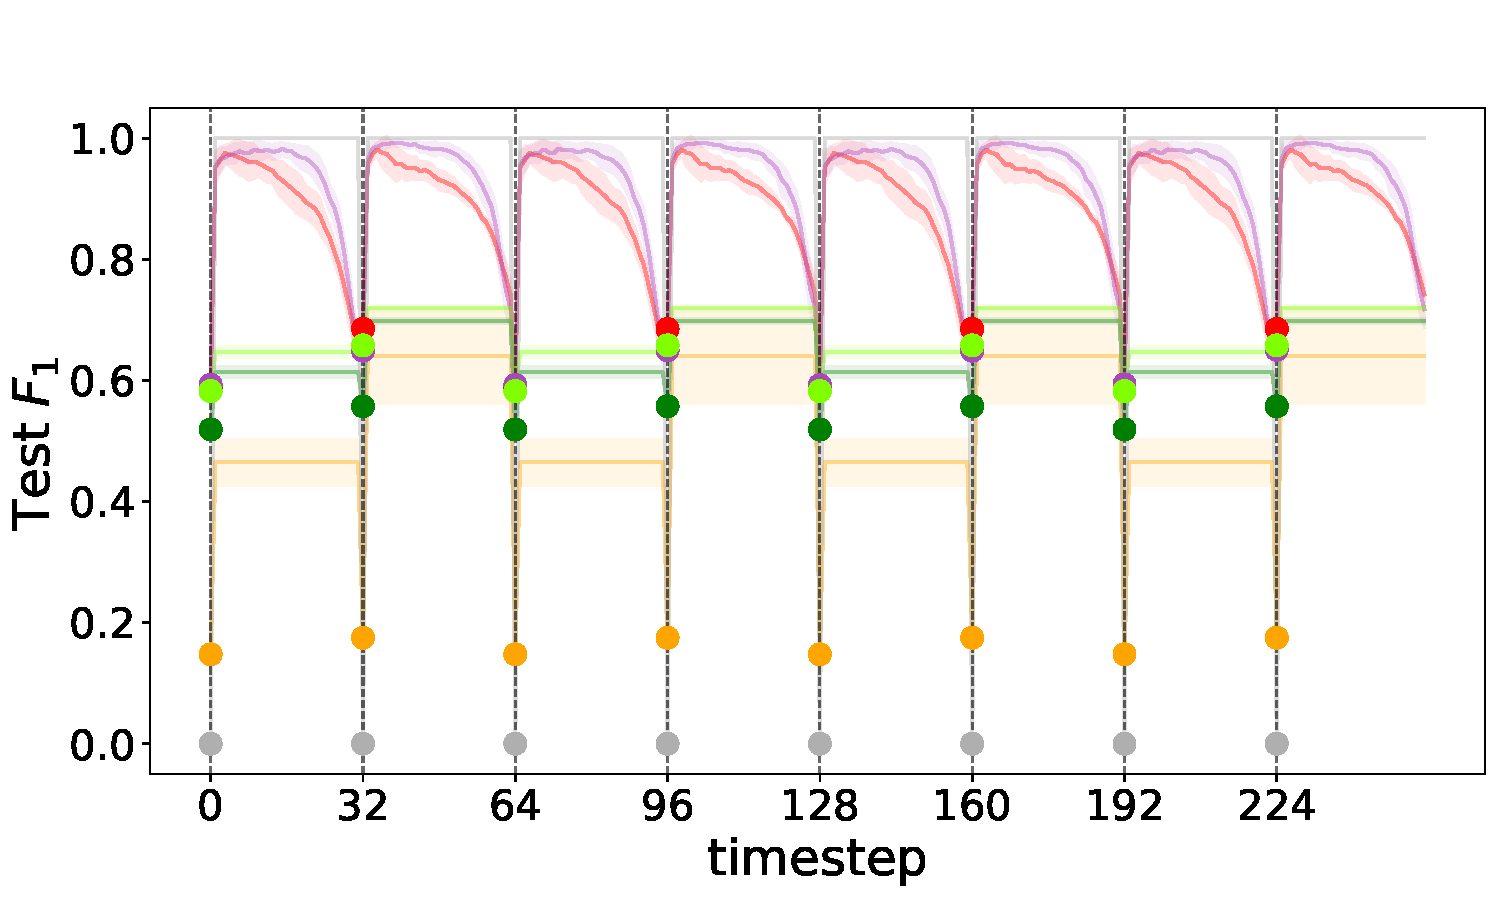
\includegraphics[width=\linewidth]{figs/periodicity/Fixed_ER/per_timestep/(2,32)DTDG_avg_f1.pdf}
        \caption{DTDG methods}
        \label{fig:sub_dtdg_det_(32,1)_per_timestep}
    \end{subfigure}
    \begin{subfigure}[b]{0.44\textwidth}
        \centering
        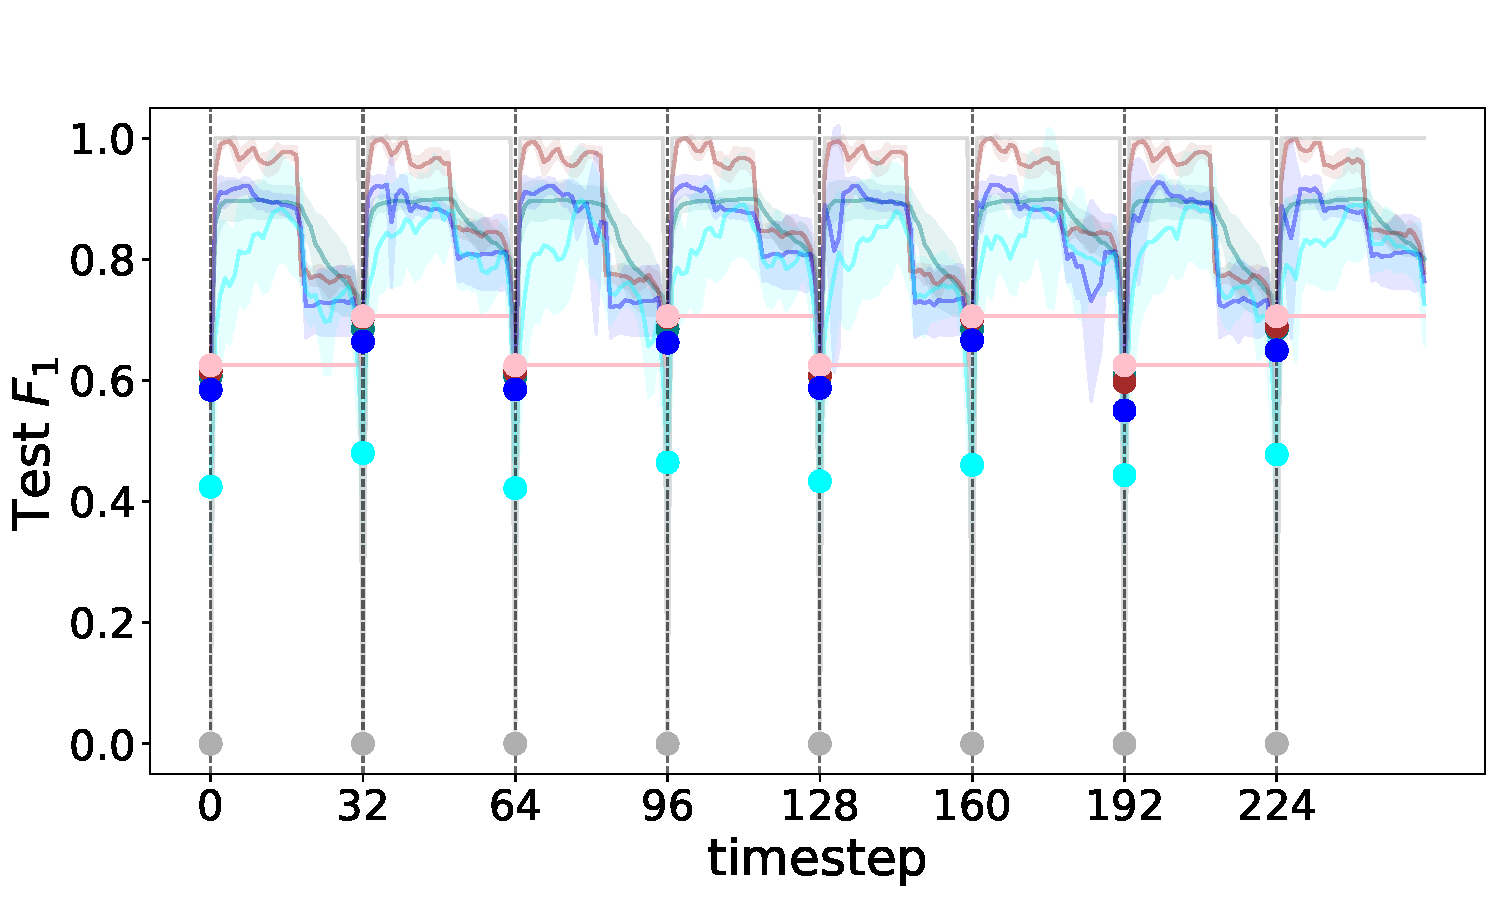
\includegraphics[width=\linewidth]{figs/periodicity/Fixed_ER/per_timestep/(2,32)CTDG_avg_f1.pdf}
        \caption{CTDG methods}
    \label{fig:sub_ctdg_det_(32,1)_per_timestep}
    \end{subfigure}
    \begin{subfigure}[b]{0.1\textwidth}
        \centering
        \raisebox{12mm}{
        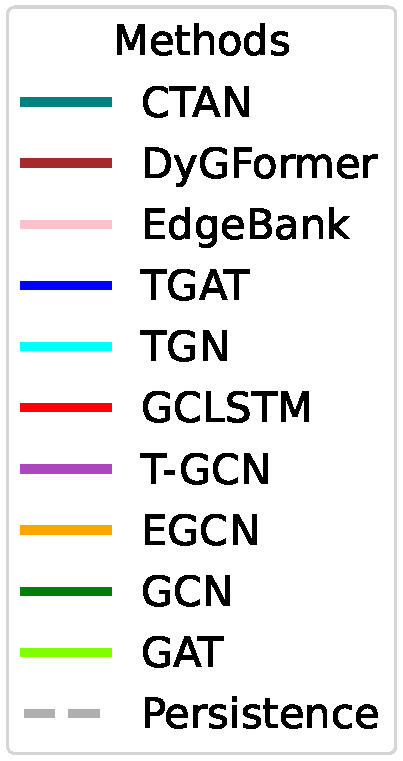
\includegraphics[width=\linewidth]{figs/legends/all.pdf}}
    \end{subfigure}
    
    \caption{The $F_1$ score at each timestep over the evaluation period is shown for DTDG (left) and CTDG (right) methods on the $\Pdet{2, 32}$ dataset.}
    \label{fig:(2,N)_per_timestep}
\end{figure}
 Figure~\ref{fig:(2,N)_per_timestep} offers a detailed, timestep-level view of model performance throughout the evaluation period. It shows that most models tend to lose performance at the start of each repetition phase and struggle to transition cleanly to the next pattern at the predefined change points (indicated by vertical lines). A notable observation is the sharp increase in performance immediately after these change points among temporal graph learning methods. This implies that these models rely on seeing the new snapshot once before adapting their predictions, which is indicative of them learning a function reminiscent of the persistence heuristic rather than properly counting. However, we note that the functions that the models learn are not \textit{exactly} equal to the persistence heuristic, as the $F_1$ score decreases between changepoints. 

\subsection{Impact of historical neighbour sampling.} \label{apendix:neighbours}
Figure~\ref{fig:(K,1)_num_neighbors_appendix} presents plots analogous to those in Figure~\ref{fig:multi_seed_neighbors}, but for additional values of $k$ in the periodicity tasks. These results offer additional insights into the impact of varying the number of neighboring samples.

In deterministic scenarios (Figures~\ref{fig:sub_num_neighbors_det_(32,1)} and \ref{fig:sub_num_neighbors_det_(64,1)}), TGAT and DyGFormer consistently exhibit robust performance, demonstrating minimal sensitivity to variations in $k$. Their $F_1$ scores remain largely stable across the tested range of neighbor samples. Conversely, TGN and CTAN display marked sensitivity to this hyperparameter. For instance, increasing k leads to substantial $F_1$ score improvements for both models, with CTAN showing gains of up to approximately 20\% and TGN similarly benefiting, underscoring their reliance on a sufficiently large neighborhood for optimal performance in these noise-free environments.

% In deterministic settings (Figure~\ref{fig:sub_num_neighbors_det_(32,1)} and ~\ref{fig:sub_num_neighbors_det_(64,1)}), TGAT and DyGFormer demonstrate robust performance with low sensitivity to the number of neighbors. In constrast, TGN and CTAN show significant improvements of up to 20\% in \( F_1 \) score, highlighting their strong sensitivity to the number of historical neighboring samples.

Under stochastic conditions (Figures~\ref{fig:sub_num_neighbors_sto_(4,1)} and \ref{fig:sub_num_neighbors_sto_(16,1)}), TGAT continues to demonstrate low sensitivity to $k$, maintaining relatively stable $F_1$ scores, akin to its behavior in the deterministic setting. DyGFormer, however, struggles significantly in the presence of noise, yielding considerably lower $F_1$ scores across all values of $k$, which suggests a lack of robustness to stochasticity in the temporal data. TGN's performance in stochastic settings appears somewhat erratic; while it benefits from more neighbors initially in $\Psto{4, 1}$, this trend does not hold consistently, as seen in $\Psto{16, 1}$ where performance degrades significantly at $k = 128$. In contrast, CTAN consistently leverages an increased number of historical neighbors, with its $F_1$ score progressively improving with larger $k$, mirroring its behavior in the deterministic tasks and indicating a capacity to filter noise or extract a clearer signal when more historical context is available.

% Figures~\ref{fig:sub_num_neighbors_sto_(4,1)} and~\ref{fig:sub_num_neighbors_sto_(16,1)} show results in the noisy (stochastic) setting. Here, TGAT maintains its low sensitivity to the number of neighbors, consistent with the deterministic case. Interestingly, DyGFormer performs poorly under noise, making it less reliable in such environments. TGN is unstable during training; increasing the number of neighboring samples does not consistently improve performance, as evident in \(\Psto{16, 1}\) with 128 neighbors. Meanwhile, CTAN continues to benefit progressively from additional historical neighbors, exhibiting the same trend observed in the deterministic setting.

\begin{figure}[H]
    % (k, 1) CTDG
    \centering
    \begin{subfigure}[b]{0.24\textwidth}
        \centering
        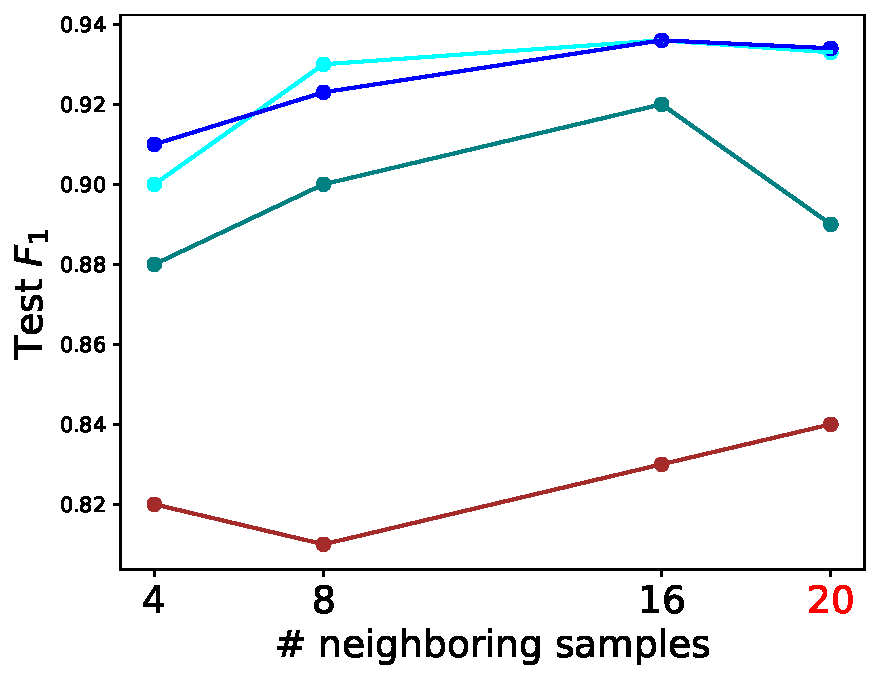
\includegraphics[width=\linewidth]{figs/periodicity/sbm_sto/V2/num_neighboring/(4, 1)(0.9, 0.01).pdf}
        \caption{$\Psto{4, 1}$}
        \label{fig:sub_num_neighbors_sto_(4,1)}
    \end{subfigure}
    \begin{subfigure}[b]{0.24\textwidth}
        \centering
        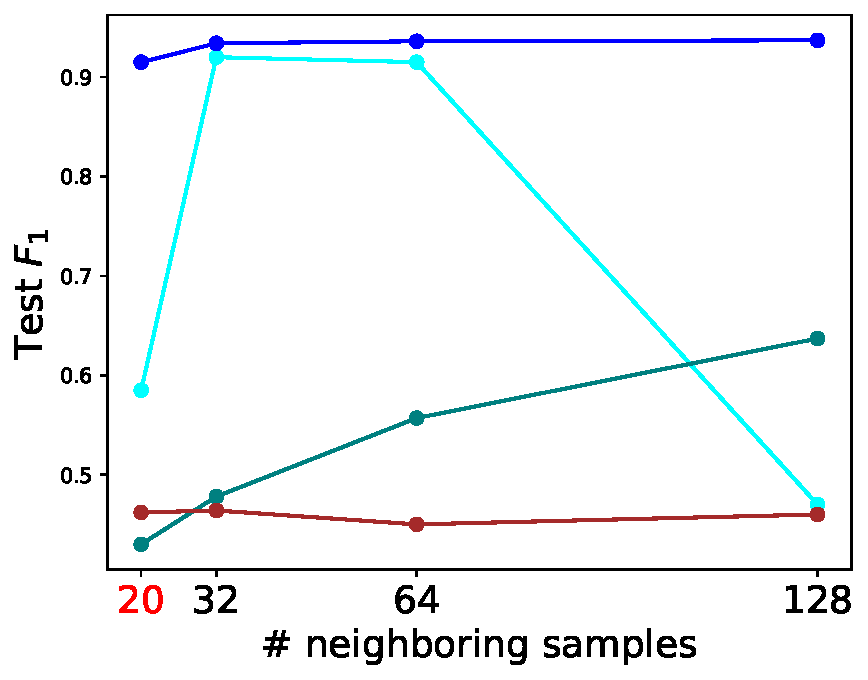
\includegraphics[width=\linewidth]{figs/periodicity/sbm_sto/V2/num_neighboring/(16, 1)(0.9, 0.01).pdf}
        \caption{$\Psto{16, 1}$}
        \label{fig:sub_num_neighbors_sto_(16,1)}
    \end{subfigure}
    \begin{subfigure}[b]{0.24\textwidth}
        \centering
        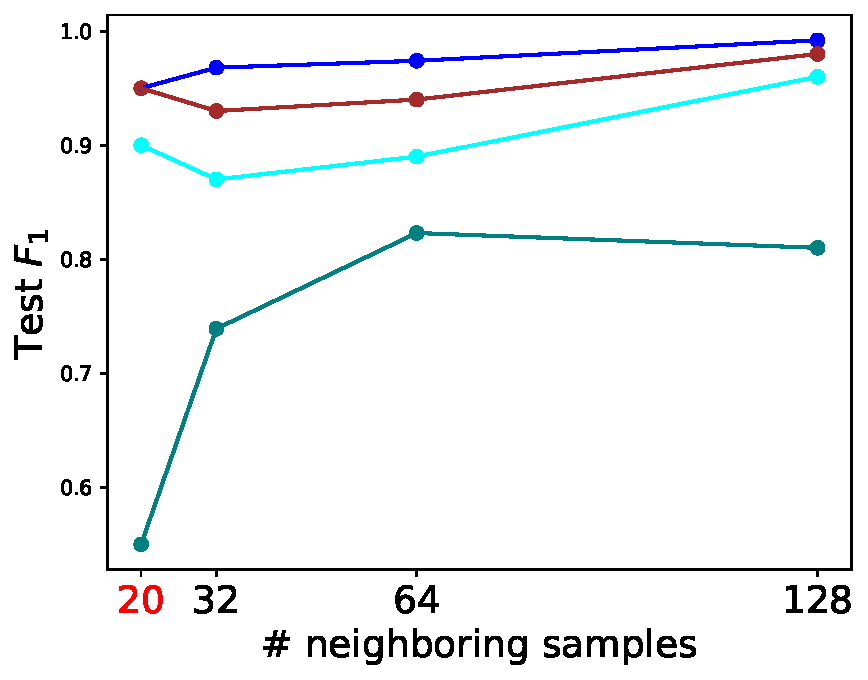
\includegraphics[width=\linewidth]{figs/periodicity/Fixed_ER/num_neighboring/(32,1).pdf}
        \caption{$\Pdet{32, 1}$}
        \label{fig:sub_num_neighbors_det_(32,1)}
    \end{subfigure}
    \begin{subfigure}[b]{0.24\textwidth}
        \centering
        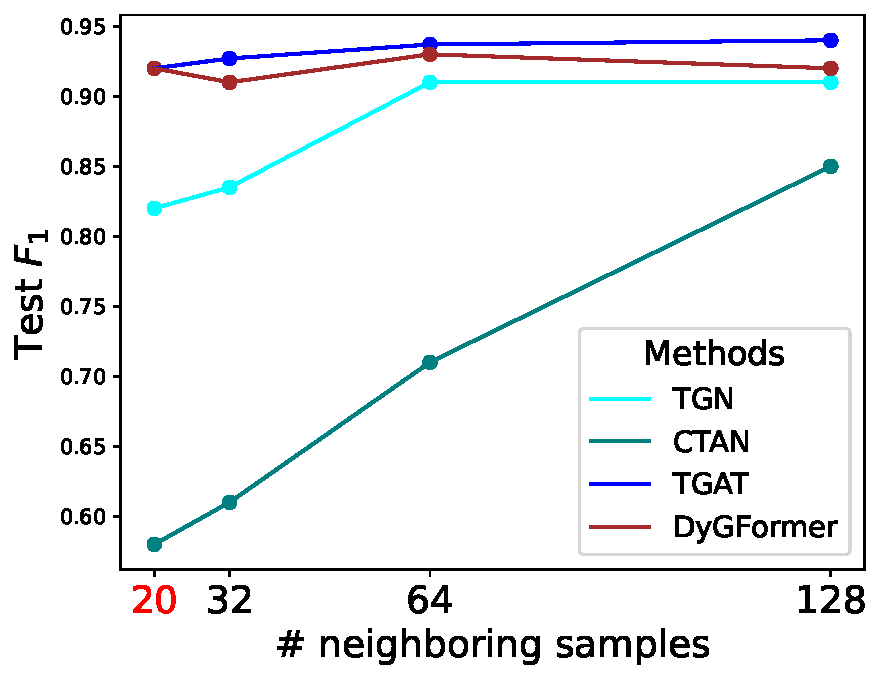
\includegraphics[width=\linewidth]{figs/periodicity/Fixed_ER/num_neighboring/(64,1).pdf}
        \caption{$\Pdet{64, 1}$}
        \label{fig:sub_num_neighbors_det_(64,1)}
    \end{subfigure}
    \caption{The impact of number of historical neighbor sampling on stochastic and deterministic periodic tasks.}
    \label{fig:(K,1)_num_neighbors_appendix}
\end{figure}

\subsection{Spatio-temporal long-range tasks (full methods)} \label{apendix:spatio_temporal_full_methods}
Figure~\ref{fig:plots_long_range_full} presents the evaluation results on spatio-temporal long-range tasks using the full set of methods, rather than the subset of top-performing models shown in \Cref{fig:plots_long_range}. In this analysis, we additionally include CTAN, EvolveGCN, GCN, and GAT. Interestingly, CTAN performs poorly across all tasks, despite its explicit design to capture long-range dependencies. GAT, on the other hand, performs reasonably well when the temporal dependency is small ($\ell=1$), suggesting that static graphs can sufficiently model simple temporal patterns. However, its performance declines sharply as the temporal dependency increases, resulting in a failure to capture both higher-order temporal and spatial dependencies.

\begin{figure}[H]
    % (k, 1) CTDG
    \centering
    \begin{subfigure}[b]{0.22\textwidth}
        \centering
        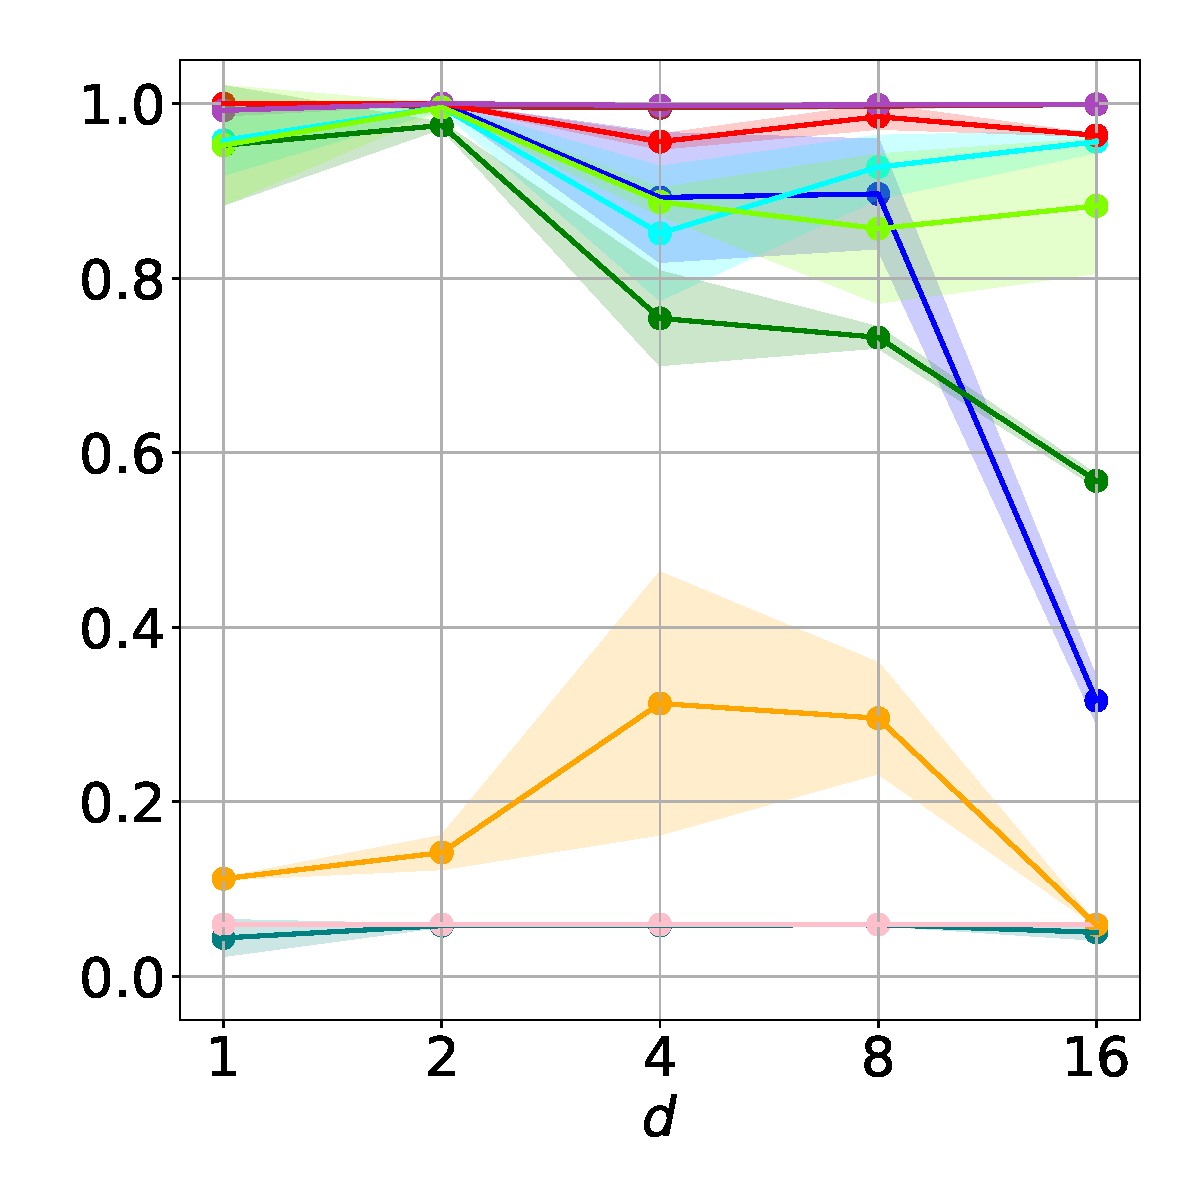
\includegraphics[width=\linewidth]{figs/long_range/fig(10, 10)/(1, d)All_Test $F_1$.pdf}
        \caption{$(\ell=1, d)$}
        \label{fig:sub_long_range_full_(1,d)}
    \end{subfigure}
    \begin{subfigure}[b]{0.22\textwidth}
        \centering
        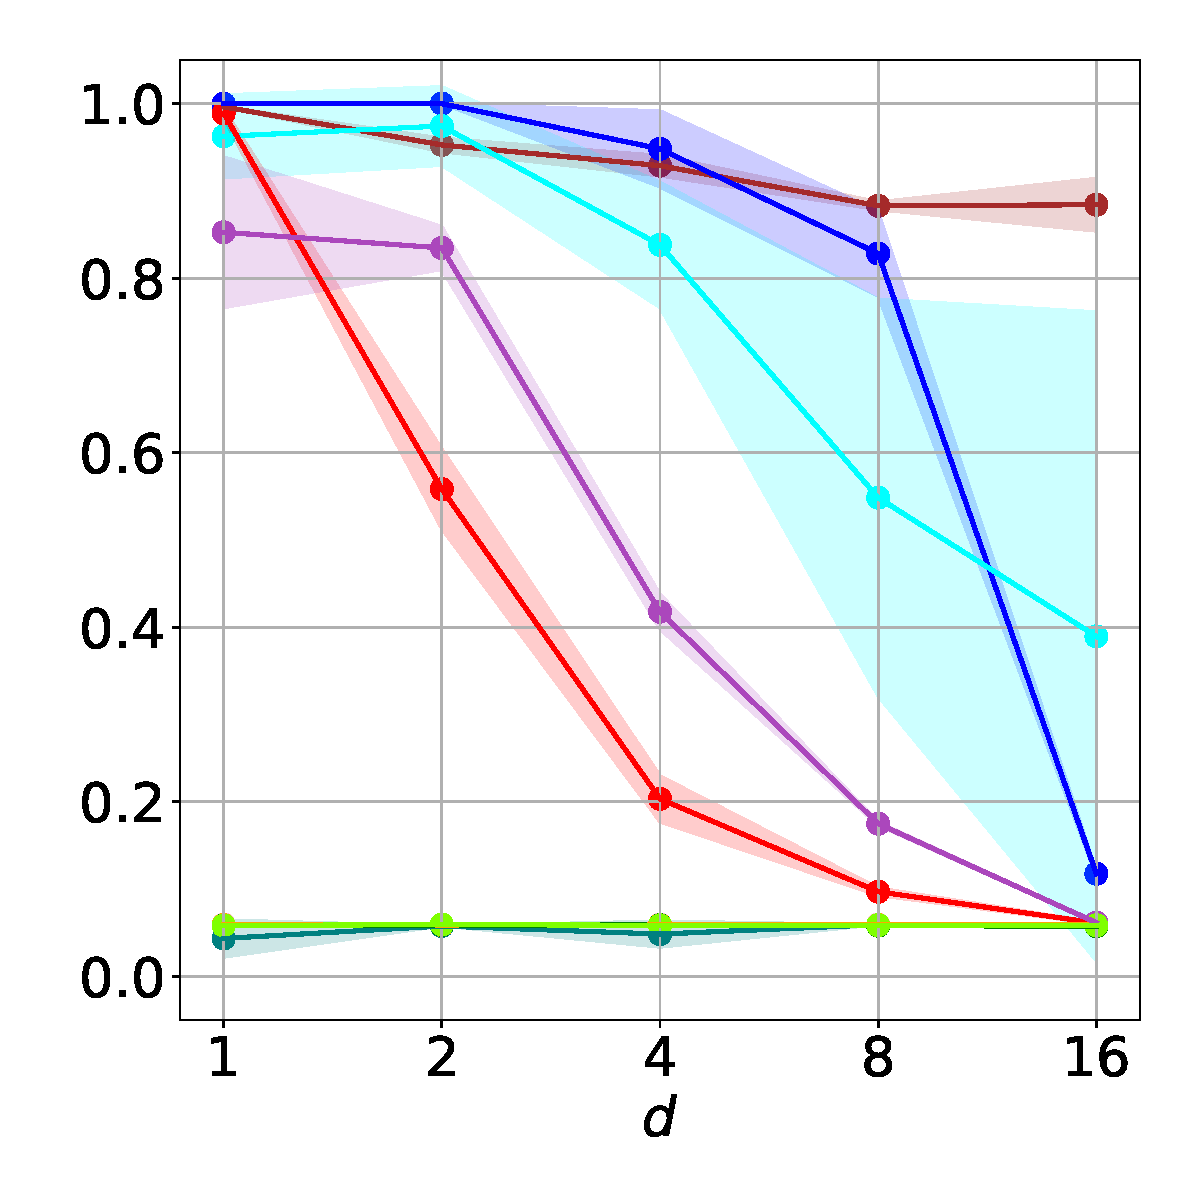
\includegraphics[width=\linewidth]{figs/long_range/fig(10, 10)/(4, d)All_Test $F_1$.pdf}
        \caption{$(\ell=4, d)$}
        \label{fig:sub_long_range_full_(4,d)}
    \end{subfigure}
    %(k, 1) DTDG
    \centering
    \begin{subfigure}[b]{0.22\textwidth}
        \centering
        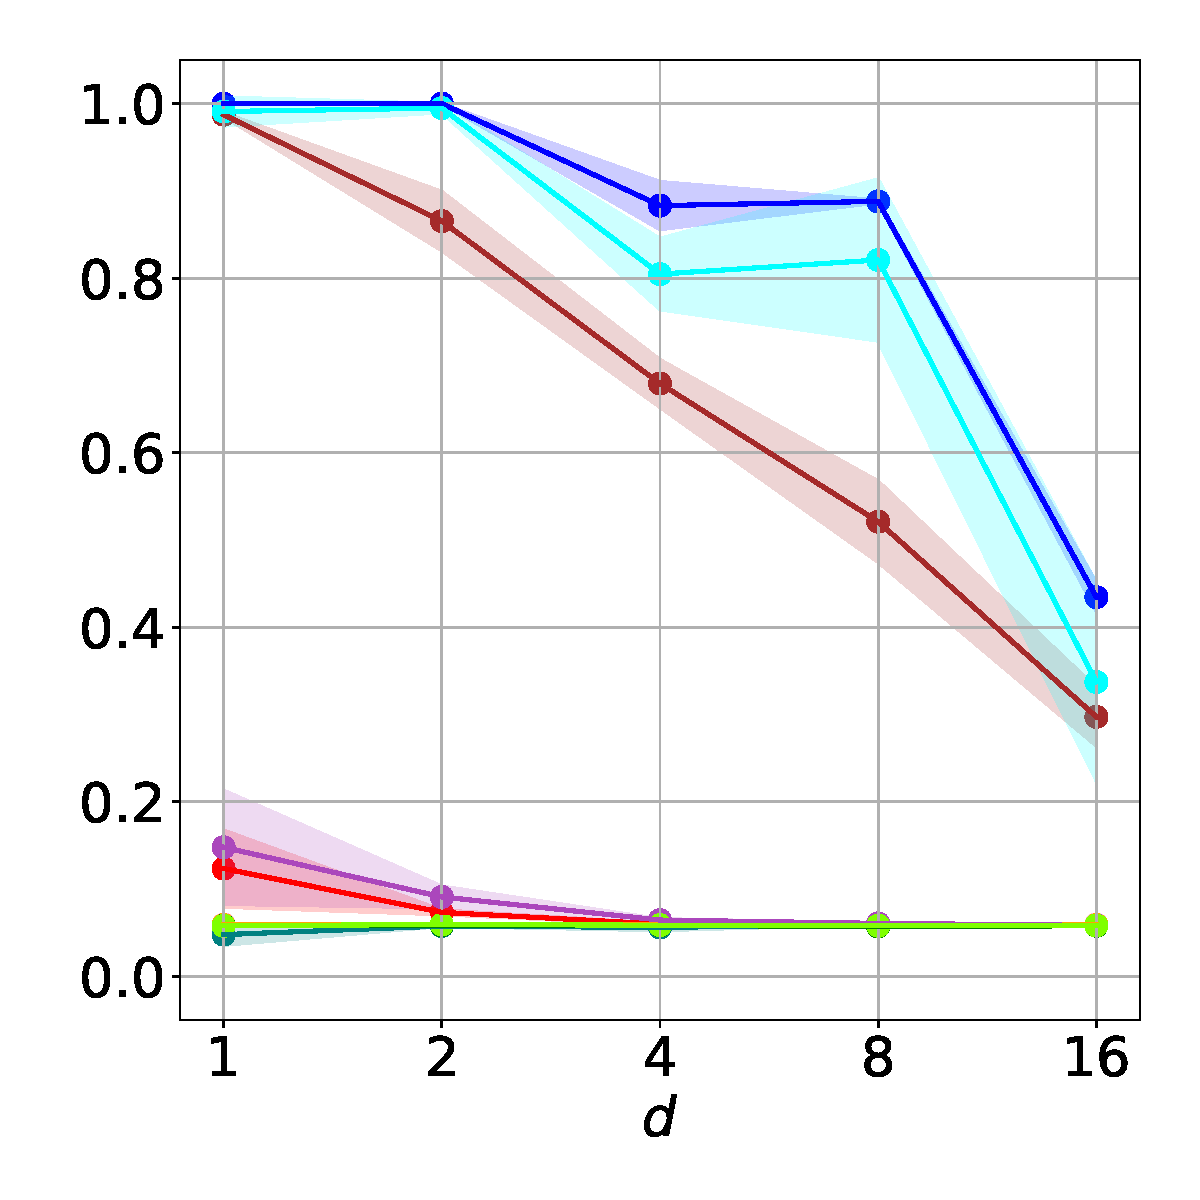
\includegraphics[width=\linewidth]{figs/long_range/fig(10, 10)/(16, d)All_Test $F_1$.pdf}
        \caption{$(\ell=16, d)$}
        \label{fig:sub_long_range_full_(16,d)}
    \end{subfigure}
    \begin{subfigure}[b]{0.22\textwidth}
        \centering
        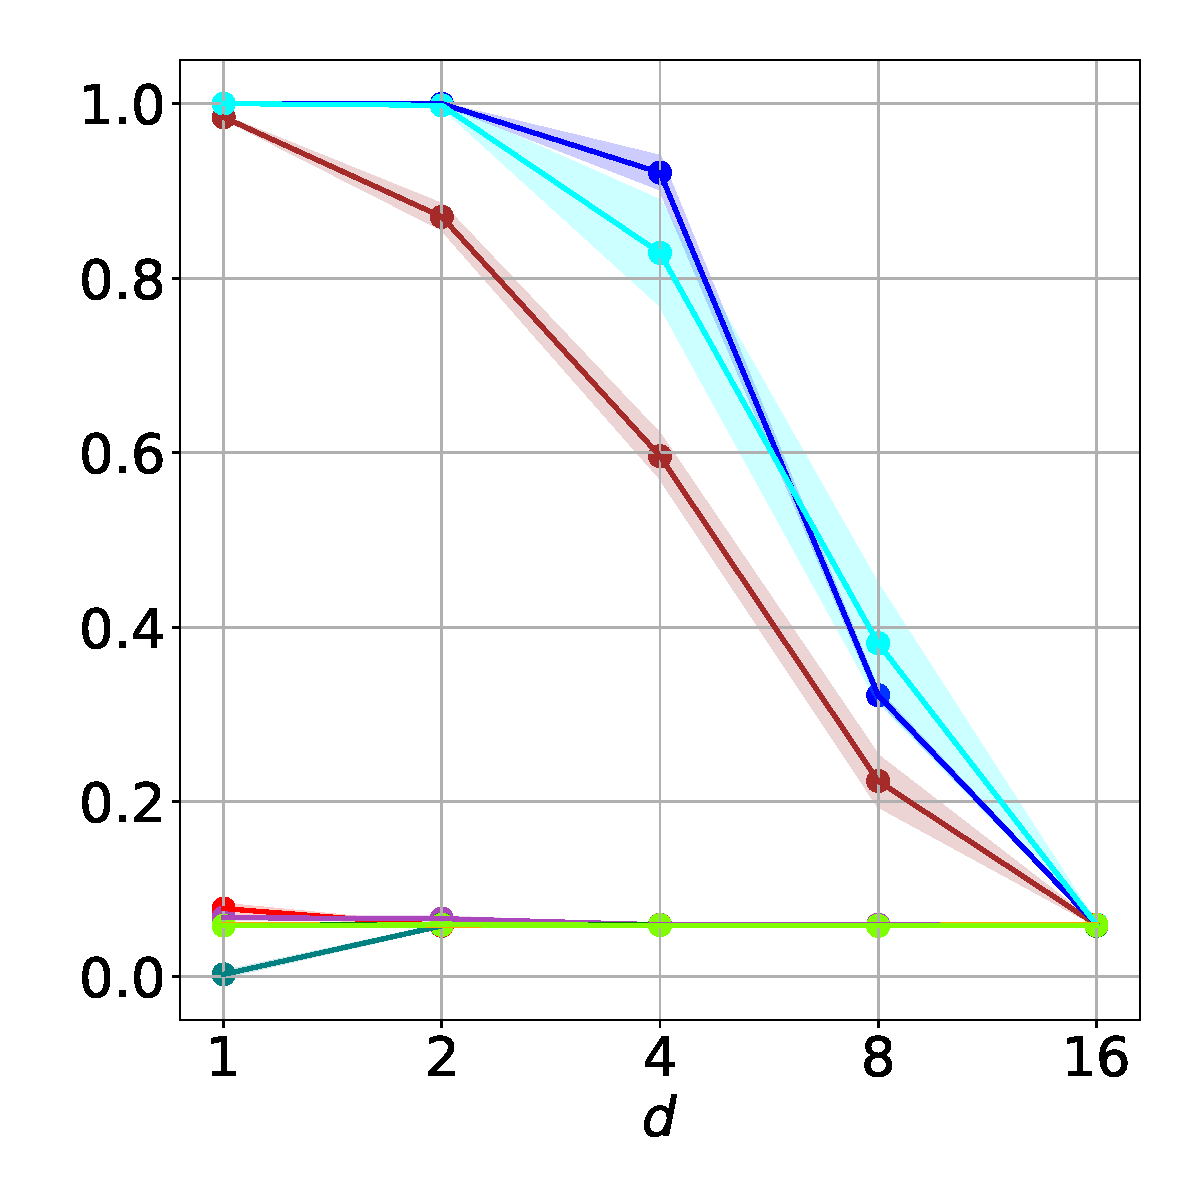
\includegraphics[width=\linewidth]{figs/long_range/fig(10, 10)/(32, d)All_Test $F_1$.pdf}
        \caption{$(\ell=32, d)$}
        \label{fig:sub_long_range_full_(32,d)}
    \end{subfigure}
    \begin{subfigure}[b]{0.08\textwidth}
        \centering
        \raisebox{15mm}{
        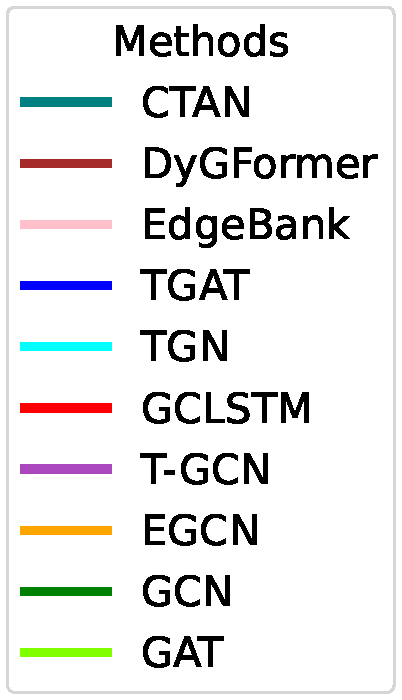
\includegraphics[width=\linewidth]{figs/legends/CTDG DTDG all w edgebank wo persistence.pdf}}
    \end{subfigure}
    
    \caption{(Full methods version) Long-range spatio-temporal tasks across varying spatial and temporal distances.}
    \label{fig:plots_long_range_full}
\end{figure}